% section/paper on sampling with sampled priors.
% \documentclass[preprint,linenumbers]{aastex631} # 6.31 fails with \align!!
\documentclass[linenumbers, onecolumn]{aastex63}
\usepackage{xcolor}

\usepackage{natbib}
\usepackage{amsmath}
\usepackage{enumitem}

\shortauthors{Bernstein et al.}

\newcommand{\ie}{\textit{i.e.}}
\newcommand{\eg}{\textit{e.g.}}
\newcommand{\E}{\mathrm{E}}
\newcommand{\eqq}[1]{Equation~(\ref{#1})}
\newcommand\gary[1]{{\color{red} \{\textbf{GMB}: #1\}}}
%\tabletypesize{\footnotesize}
\newcommand{\vecc}{\ensuremath{\mathbf{c}}}
\newcommand{\vecq}{\ensuremath{\mathbf{q}}}
\newcommand{\vecs}{\ensuremath{\mathbf{s}}}
\newcommand{\vecn}{\ensuremath{\mathbf{n}}}
\newcommand{\vecu}{\ensuremath{\mathbf{u}}}
\newcommand{\vecv}{\ensuremath{\mathbf{v}}}
\newcommand{\hatc}{\ensuremath{\hat{\mathbf{c}}}}
\newcommand{\vecP}{\ensuremath{\mathbf{P}}}
\newcommand{\covm}{C}
\newcommand{\matA}{\ensuremath{A}}
\newcommand{\matD}{D}
\newcommand{\matE}{E}
\newcommand{\matF}{F}
\newcommand{\matG}{G}
\newcommand{\matI}{I}
\newcommand{\matT}{T}
\newcommand{\matX}{X}
\newcommand{\matY}{Y}
\newcommand{\matV}{V}
\newcommand{\matLam}{\Lambda}
\newcommand{\proj}{P}  % Projection matrix
\newcommand{\jac}{J}   % Jacobian
\newcommand{\ident}{I}  % identity
\newcommand{\DD}{\Delta_D}
\newcommand{\likeli}{\mathcal{L}}
\newcommand{\trace}{\text{Tr}}
\begin{document}

\title{Sampling Bayesian probabilities given only sampled priors}

\author[0000-0002-8613-8259]{Gary M. Bernstein}
\affiliation{Department of Physics and Astronomy, University of Pennsylvania, Philadelphia, PA 19104, USA}
\email{garyb@upenn.edu}

\author{Troxel,William,Boyan,Giulia,Alex Amon,Alex Alarcon,\ldots}

\begin{abstract}
	\vspace{0.2in}
A typical Bayesian inference on the values of some parameters of
interest $\vecq$ from some data $D$ would run a Markov Chain (MC) to sample
from the posterior $p(\vecq,\vecn | D) \propto \likeli(D | \vecq,\vecn)
p(\vecq) p(\vecn),$ where $\vecn$ are some nuisance parameters.  In
many cases, the nuisance parameters are high-dimensional, and their
prior $p(\vecn)$ is itself defined only by a set of samples that have
been drawn from some other MC.  Two problems arise: first,
the MC for the posterior will typically require evaluation of
$p(\vecn)$ at arbitrary values of $\vecn,$ \ie\ one needs to provide a
density estimator over the full $\vecn$ space from the provided
samples.  Second, the high dimensionality of $\vecn$ hinders both the
density estimation and the efficiency of the MC for the posterior.  We
describe a solution to this problem: a linear compression of the
$\vecn$ space into a much lower-dimensional space $\vecu$ which
projects away directions in $\vecn$ space that cannot appreciably
alter $\likeli.$ The algorithm for doing so is a slight modification
to principal components analysis, and is less restrictive on
$p(\vecn)$ than other proposed solutions to this issue.
We demonstrate this ``mode projection'' technique using the analysis
of 2-point correlation functions of weak lensing fields and galaxy
density in the \textit{Dark Energy Survey}, where $\vecn$ is a binned representation of the redshift distrbution
$n(z)$ of the galaxies.
\end{abstract}
\reportnum{}

\section{Motivation} \label{sec:intro}

Consider an inference in which we have a vector of observable summary
statistics \vecc\ that we are using to constrain a set of parameters of
interest \vecq.  There is a model $\hatc(\vecq,\vecn)$ for the
observables which involves the parameters of interest, but also a
vector \vecn\ of nuisance parameters.  
We wish to characterized the Bayesian posterior probability
\begin{equation}
  p(\vecq | \vecc) \propto \int dn\, \likeli(\vecc | \vecq, \vecn) p(\vecq) p(\vecn),
\label{eq:posterior}
\end{equation}
where $\likeli(\vecc | \vecq, \vecn)$ is a known likelihood function
of the data, and $p(\vecq)$ and $p(\vecn)$ are priors on the
parameters.  This posterior is complex enough that it requires
approximation by the output of a Markov chain (MC) wandering across the space $(\vecq,\vecn).$

The scenario we address here is when \emph{the prior $p(\vecn)$ is itself known only from a set of samples of $\vecn$ from this distribution.} Most MC samplers require that the posterior be an evaluable function of any value of the parameters, and it is the general task of density estimators to convert the samples of $\vecn$ into an evaluable $p(\vecn).$  But when \vecn\ is of high dimension, two problems arise: first, there may be insufficient available samples to create a viable density estimator; second, sampling of the posterior in (\ref{eq:posterior}) becomes infeasible if the MC must traverse a high-dimensional space.

A concrete example, which motivated this development,
is when the observable data \vecc\ are the binned 2-point correlation functions of
cosmic fields derived from a catalog of galaxies; the parameters of
interest are cosmological quantities such as $\Omega_m, \sigma_8,$
etc.; and the nuisance parameters $\vecn$
include the coefficients of some linear expansion of the redshift distributions $n(z)$ of the galaxies being observed:
\begin{equation}
  n(z) = \sum_{k=1}^{M} n_k b_k(z).
  \label{eq:nzbasis}
\end{equation}
The $b_k$ are a set of predetermined basis functions for the redshift
distribution.  In our case there are 10 distinct galaxy populations to be characterized, leading to $O(1000)$ parameters $n_k$ to be considered.

One approach would be to run a new MC chain over \vecq\ for each of the samples we have of \vecn, and then concatenate these to effect marginalization over \vecn.  This is clearly infeasible if a large number of \vecn\ samples are needed to characterize the prior in this space.

Facing this problem for the cosmological analyses of the 3-year data (Y3)
of the \textit{Dark Energy Survey} (DES),
\citet{hyperrank} devised a scheme whereby
the samples of \vecn\ are placed in a grid within some $M$-dimensional
unit hypercube $\mathcal{H}$.  The coordinates \vecu\ within the hypercube
are considered the compressed parameters of $n(z),$ and the
decompression function
$\hat{\vecn}(\vecu)$ outputs the $\vecn_\alpha$ sample at the nearest grid point to
  \vecu.  This solves the problem of creating a continuous \vecu\
  domain, and maintains the equal prior probability of each \vecn\
  sample, but the function \emph{output,} and the resultant likelihood
  function of \vecu, are discontinuous.
Various strategies are proposed to assign the $\vecn_\alpha$ to the grid points in
$\mathcal{H}$ based on summary statistics, to reduce the
discontinuities.  But the function is never smooth.
As a consequence, many MC samplers become quite inefficient in
sampling of the cosmological posterior.  In particular, samplers such as \textsc{MultiNest} that assume continuity are rendered nearly non-functional.  As a result, the Y3 cosmological priors could not be evaluated with this method.  Instead, the \vecn\ samples were not used, and an \textit{ad hoc} $p(\vecn)$ was adopted which allowed only shifts and dilations of the mean $n(z)$ of the \vecn\ samples.

A more rigorous and extremely efficient method of marginalizing over high-dimensional nuisance parameters was proposed by \citet{hans}, for the case where the following restrictions apply:
\begin{enumerate}
\item The likelihood of the observable \vecc\ is normal, $\vecc \sim \mathcal{N}( \hatc, \covm_c),$ with $\covm_c$ fixed.
\item The prior $p(\vecn)$ can also be assumed to be normal, with a mean and covariance matrix $\covm_n$ that in our case could be assigned from the mean and covariance of the samples of \vecn\ we are given.
\item The model \hatc\ can be linearized in \vecn\ about fiducial values $\vecq_0, \vecn_0$ without loss of accuracy exceeding measurement errors, with the derivatives independent of \vecq.
\end{enumerate}
Under these conditions, \citet{hans} show that the marginalization over \vecn\ is equivalent to adding terms to $\covm_c,$ such that any MC process need not sample \vecn\ at all.

We describe here an approach that is algebraically similar to that of \citet{hans}, but does not require 2nd condition of Gaussianity for the nuisance prior.  Our approach is to seek a linear compression of \vecn\ into a lower-dimensional set of parameters \vecu\ that projects away variations in \vecn\ that do not influence the likelihood $\likeli.$  Standard density estimators can then be applied to the \vecu\ values implied by the known \vecn\ samples to yield a prior $p(\vecu)$ that can be used for the MC chain of the cosmological posterior.  The model \hatc, and hence $\likeli,$ will be continuous over this low-dimensional \vecu\ space, and marginalization over \vecu\ will yield posterior probabilities very close to marginalization over the original \vecn.  

\section{Derivation}\label{sec:deriv}
We assume that we do have a multivariate normal likelihood for the
observables \vecc\, with the mean being some model
$\hatc(\vecq,\vecn)$ and a fixed covariance matrix $\covm_c.$ In this
section we will assume that the \vecn\ vectors have been shifted by
the mean of the samples $\vecn_0 \equiv \left\langle \vecn_\alpha \right\rangle$ so
that the new \vecn\ has zero mean.
We seek some function $\hat{\vecn}(\vecu)$ of a lower-dimensional
vector \vecu\ which can be substituted for \vecn\ and yield nearly the
same likelihood function for any \vecn\ in the domain spanned by the
samples $\vecn_\alpha,\; \alpha\in 1\ldots N_\alpha.$
This means we want a map $\vecn_\alpha\rightarrow
\vecu_\alpha \rightarrow \hat{\vecn}_\alpha$ such that replacing $\vecn$ with
$\hat\vecn$ alters the cosmological inference by much less than the
other uncertainties in the model or data.  We will implement this by minimizing the
distance in the space $\vecc$ between the
model generated by $\vecn$ and that by $\hat\vecn$, using the
observations' covariance matrix $\covm_c$ as a metric for the
distance.\footnote{More precisely, the inverse of the covariance
  matrix is the metric.}  This is equivalent to the $\chi^2$ of the difference
between the original and compressed models for the data:
\begin{equation} \left\langle \chi^2 \right\rangle
=  \frac{1}{N_\alpha} \sum_\alpha
                                            \left[ \hatc(\vecq,\vecn_\alpha) - \hatc(\vecq,\hat{\vecn}_\alpha) \right]^T
                                            \covm_c^{-1}
                                            \left[ \hatc(\vecq,\vecn_\alpha) - \hatc(\vecq,\hat{\vecn}_\alpha) \right].
\label{eq:chisq}
\end{equation}
If the data are in fact drawn from the model $\hatc(\vecq,\vecn)$ with
a Gaussian likelihood, then this is also the mean shift in $-2\log\likeli$
from the compression.  It is \emph{not}, however, equal to the mean
shift of the overall log of the posterior in
\eqq{eq:posterior}---rather, $\left\langle\chi^2\right\rangle$ is serving as a
proxy for the true log-likelihood shift. 

We next assume that the compression is linear, $\hat\vecn=\matX\vecn,$
for some matrix that is idempotent ($\matX\matX = \matX$).  If this is
true, then the contribution to \eqq{eq:chisq} at lowest order in
$\vecn-\hat\vecn$ is
\begin{equation}
  \left\langle \chi^2 \right\rangle = \frac{1}{N_\alpha} \sum_\alpha
  \left[ (\matI-\matX)\vecn_\alpha\right]^T \matF  \left[ (\matI-\matX)\vecn_\alpha\right]
  \label{eq:linearized}
\end{equation}
where we use the Jacobian matrix of the model $\hatc$ to define
\begin{equation}
  \matF \equiv
  \left[\frac{\partial\hatc}{\partial\vecn}\right]_{\vecq_0, \vecn_0}
  \covm_c^{-1} \left[\frac{\partial\hatc}{\partial\vecn}\right]_{\vecq_0,
    \vecn_0}^T.
\label{eq:fisher}
\end{equation}
This quantity is also the Fisher matrix giving the information
provided by the observations $\vecc$ about the nuisance parameters
\vecn.  In many cases this matrix will be
rank-deficient and/or poorly conditioned, since the observables are not
likely to be very informative on $\vecn$---if they were, we might not be
concerned with establishing a prior on $\vecn$ to begin with.
Fortunately, we will not require the inverse of $\matF$ in our algorithm.

The optimization implied by \eqq{eq:linearized} is the same as in
familiar Principal Components Analysis (PCA), aside from the presence
of the $F$ matrix, which in essence defines a new metric for the
variance to be captured by the principal components.  Our solution will follow the typical derivation
for PCA, but with an additional variable transformation to compensate
for the presence of $\matF.$

Since $\matX$ is idempotent, we can write
\begin{align}
  \matX & = V_X \proj_M V_X^T, \\
  \matY \equiv \matI-\matX & = V_X \proj_{-M} V_X^T,
\end{align}
where $V_X$ is unitary and the projection matrix $\proj_M$ is defined as
\begin{equation}
  \left(\proj_M\right)_{ij} \equiv
\begin{cases}
                                            1,  &  i=j\le M \\
                                            0,  & \text{otherwise}
\end{cases}
\end{equation}
and $\proj_{-M}=\matI-\proj_M.$  For a chosen rank $M$ of the
transformation matrix $X$, our task becomes to identify the
eigenvectors $V_X$ that minimize
\begin{align}
  \left\langle \chi^2\right\rangle & = \frac{1}{N_\alpha} \sum_\alpha
  \left[ \matY \vecn_\alpha\right]^T \matF  \left[\matY
                                     \vecn_\alpha\right] \\
       & = \trace \left[ \covm_n V_X \proj_{-M} V_X^T \matF V_X
         \proj_{-M} V_X^T \right], \\
  C_n & \equiv \left\langle \vecn \vecn^T \right\rangle.
\end{align}
This optimization is easier if we transform first the systematic variables to
$\vecn^\prime =\matT\vecn$ such that $\covm_{n^\prime}=\matI$, \ie\
make the elements of $\vecn$ uncorrelated and unit-variance.  This
is accomplished by finding the eigensystem $\covm_n=\matV_n \matLam_n
\matV_n^T$ and setting $\matT = \matLam_n^{-1/2} \matV_n^T$.  With
this transformation, we are now seeking a different unitary matrix
$\matV_{X^\prime}$ that minimizes
\begin{align}
  \left\langle \chi^2\right\rangle & = \trace \left[ \matI
    V_{X^\prime} \proj_{-M} V_{X^\prime}^T \left[ (T^{-1})^T \matF
      T^{-1} \right] V_{X^\prime} 
    \proj_{-M} V_{X^\prime}^T \right] \\
  & = \trace \left[ \proj_{-M} V_{X^\prime}^T \matV_G \matLam_G \matV_G^T
    V_{X^\prime} \proj_{-M} \right],
  \label{eq:mintr}\\
  \matG \equiv \left(T^{-1}\right)^T \matF   T^{-1} & = \matLam_n^{1/2} \matV_n^T
  \matF \matV_n \matLam_n^{1/2} = \matV_G \matLam_G \matV_G^T.
  \label{eq:defG}
\end{align}
The last line defines a transformed Fisher matrix $\matG$ and its
(non-negative) eigensystem.  Examination of \eqq{eq:mintr} reveals that this quantity
is minimized if the elements of the unitary matrices satisfy
$\matV_{X^\prime}^T \matV_G = \matI \; \Rightarrow \; \matV_{X^\prime} = \matV_G,$ and the eigensystem of $G$ is placed
in order of decreasing eigenvalue $\lambda^G_i.$ The
elements surviving the project functions yield
\begin{equation}
  \left\langle \chi^2\right\rangle = \sum_{i>M} \lambda_i^G.
  \label{eq:chiresid}
\end{equation}
In other words each eigenvalue of the matrix $\matG$ in \eqq{eq:defG}
gives the contribution to $\left\langle\chi^2\right\rangle$ of one
projection (mode) of $\vecn.$

Transforming the solution back into the space of $\vecn$ yields
\begin{align}
  \matX & = \matT^{-1} \matV_G \proj_M \matV_G^T \matT \\
\label{eq:DE}
   & = \left[ \matV_n^T \matLam_n^{1/2} \matV_G \proj_M \right] \left[
     \proj_M \matV_G^T \matLam_n^{-1/2} \matV_n^T \right] \\
        & \equiv \matD \matE.
\end{align}
We thus obtain our optimal encoding/compression using the nonzero rows of matrix
$\matE$ to give
\begin{equation}
  \vecu_\alpha = \matE \vecn_\alpha
  \label{eq:uu}
\end{equation}
and the decoding/reconstruction of the systematic variables as
\begin{equation}
  \hat\vecn_\alpha = \matD \vecu_\alpha.
  \label{eq:UU}
\end{equation}
One can confirm that this procedure yields a compressed representation
$\vecu$ such that $\covm_u = \matI_M,$ the $M$-dimensional
identity matrix.

The previous derivation ignores the possibility that $\covm_n$ is
singular or nearly so, such that taking $\matLam_n^{-1/2}$ in
\eqq{eq:DE} is not possible.  Indeed in our application, it is
\emph{required} that $\covm_n$ be singular, because we have a sum
normalization constraint on the initial $\vecn_\alpha$ values.  Any
such (nearly) zero element $j$ of $\matLam_n$ has a corresponding
eigenvector $\vecv_j$ of the $\vecn$ space which has zero amplitude
in all of the input samples $\vecn_\alpha,$ so that the $\vecn$ are
confined to a subspace---the reconstructed $\hat\vecn$ should also be.
The compressed
representations $\vecu_\alpha$ and reconstructed $\hat\vecn_\alpha$
should therefore be unaffected by the presence of any $\vecv_j$
component.  This can be accomplished in \eqq{eq:DE} by setting element
$j$ of $\matLam_n^{-1/2}$ to zero, as is typically done during
solutions of least-squares problems using singular value
decompositions.

In summary, the procedure for dimensional reduction is:
\begin{enumerate}
  \item Obtain the Fisher matrix $\matF$ of the system defined in
    \eqq{eq:fisher} using derivatives about the mean sample $\vecn_0,$
    plus the covariance matrix $\covm_n$ of the samples.
  \item From the eigensystem $(\matLam_n,\matV_n)$ of $C_n$, form the
    matrix $G$ defined in \eqq{eq:defG} and get its eigensystem
    $(\matLam_G,\matV_G).$  Place the eigenvalues in descending order.
  \item Choose the size $M$ of the compressed representation to be the
    minimum that keeps the $\left\langle\chi^2\right\rangle$ value in
    \eqq{eq:chiresid} below a chosen threshold, presumably $\ll 1.$
  \item The encoding matrix $E$ and decoding matrix $D$ are formed as
    in \eqq{eq:DE}, taking the inverse $\matLam_n^{-1/2}$ to be zero
    for any eigenvalues that are zero (or within roundoff errors).
  \item Compress all incoming (mean-subtracted) samples using
    \eqq{eq:uu}.  The resulting $\vecu$ values will have
    have unit covariance matrix and zero mean.
  \item Construct a continuous density estimator in $\vecu$ space that
    mimics the finite sample distribution.  If the distribution is
    normal, this becomes the multidimensional unit normal.  There
    is, however,  no \textit{a priori} reason that this must be the case,
    and something like a normalizing flow may be needed to
    approximate this lower-dimensional representation of the prior.
  \item Sample over $\vecu$ space in the Markov Chain that is sampling the
    posterior on the parameters of interest $\vecq,$ using \eqq{eq:UU}
    to transform each sample back into a $\hat\vecn$ vector.
  \end{enumerate}
  
The ability to accomodate non-Gaussian distributions of the
nuisance-parameter space is the principle
advantage of our method over the single-step covariance-inflation
method of \citet{hans}.
But even if the \vecu\ prior is well approximated as multivariate normal,
there are practical advantages of compressing the nuisance 
variables and retaining them in the cosmological Markov chain rather
than using the covariance-inflation method for analytic
marginalization.  One can, for example, examine the posterior
distributions of \vecu\ and see if they are at the edges of the prior,
which would potentially indicate an inconsistency between the data and
the prior.
  

\section{Application}\label{sec:app}
As an example of the application of this straightforward dimensional
reduction to a high-dimensional nuisance parameter, we examine the
redshift distribution of one of the bins of ``Maglim''  galaxies used
as a lens population and clustering tracer in the Year 6 analysis of
the \textit{Dark Energy Survey (DES)} galaxy catalogs.  Each
Maglim bin's members are selected with cuts on galaxy fluxes and
colors in an attempt  to generate a sample that is confined to a
particular redshift range, as described in \citet{y6gg}.  Once each bin's
sample is chosen, a combination of 
photometric techniques \citep{y6pz} and clustering information
\citep{y6wz} are used to generate samples from the true $n(z)$
distributions of its members.
In the baseline case,
there are 6 cosmological parameters of interest, $\vecq = \{\Omega_m,
\Omega_b, \sigma_8, h, n_s, m_\nu\}.$   The nuisance vector $\vecn$
has 5--10 parameters in each of the following categories: galaxy
biases with respect to matter; intrinsic alignments of galaxy shapes
with the tidal field of the mass; and multiplicative errors in the
measurement of galaxy shear.  The $n(z)$ for each galaxy bin
is
described by \eqq{eq:nzbasis} with 80 coefficients spanning $0<z<4$ at
intervals of $\Delta z=0.05.$ If all of these coefficients, for each
galaxy sample, were allowed to vary, the parameter space for inference would be grow more
than 10-fold.  The inference would become infeasible even if a
reliable density estimator over the 80-dimensional space could be
created from the $\approx3000$ samples available to characterize each
$n(z).$ 

Thus we turn to the modal projection technique herein to reduce the
dimensionality to those directions in $\vecn$ space in which the samples span a large
enough range to alter the $\hatc(\vecn)$ at detectable levels. 

The observable quantities $\vecc$ whose modeling depends upon the these nuisance
parameters are the angular autocorrelation $w(\theta)$ of the sample
members, and the cross-correlations $\gamma_t^{(s)}(\theta)$ between
this sample's positions and the weak gravitational lensing shear
observed on the samples $1\le s \le 4$ of source galaxies.  The
derivatives of the model for each observable, and the expected
covariance, are calculated from theory with the tools described in
\citet{y6model}.

\begin{figure}
  \center
  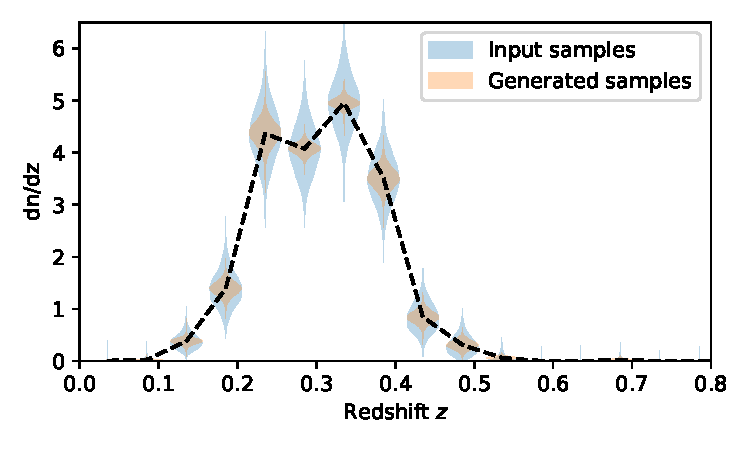
\includegraphics[width=0.6\textwidth]{violin.pdf}
\caption{Violin plots for the redshift probability distribution $n(z)$
  of galaxies in lens bin 1 for the DES Y6 analysis.  The blue regions
  show the distributions for the samples of $\vecn$ derived from
  photometric and clustering information.  The orange violins are for
  $\vecn$ values drawn defined by (1) compressing the original $\vecn$
  into 5 modes with coefficients $\vecu,$ then (2) drawing values of
  $\vecu$ from unit normal distributions and transforming them to
  match the $\vecu$ 1d distribution of the input samples.  The dashed
  line connects the mean values of $n(z),$ which are the same for
  generated samples as for the input samples, by construction.
  Although the $n(z)$ functions are calculated out to $z=4,$ we
  truncate this and other plots at lower $z$ to emphasize the
  lower-redshift regime where this bin's galaxies are primarily found.}
  \label{fig:violins}
\end{figure}

We present results for mode-compression sampling of the $n(z)$
parameters for the lowest-redshift bin.  Figure~\ref{fig:violins}
plots the distributions of the individual elements of $n(z)$ in the
input 3000 samples.  As per the procedure desribed in this paper, the
mean \vecn\ is subtracted from each sample and the covariance
$\covm_c$ computed.  This is then combined with the
derivatives and covariance matrices of the observables $\vecc$ to
calculate the decomposition in \eqq{eq:defG}.

\begin{figure}
  \center
  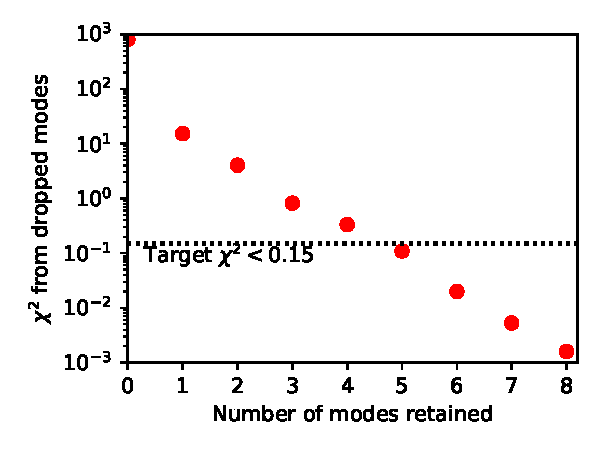
\includegraphics[width=0.6\textwidth]{chiresids.pdf}
\caption{The size of the $\chi^2$ of modeling error attributable to compressing the
  $\vecn$ samples down to $M$ modes is plotted vs $M$.  The values
  drop exponentially with $M,$ and our chosen criterion of
  $\chi^2<0.15$ is attained with $M=5$ for this bin's $n(z).$}
  \label{fig:chiresid}
\end{figure}

Figure~\ref{fig:chiresid} plots the values of unmodelled
$\chi^2$ vs the dimension $M$ of the compressed space, as per
\eqq{eq:chiresid}.  This modelling error induced by compression drops
exponentially with the number of retained modes, and our chosen criterion of
$\chi^2<0.15$ is attained with $M=5$ modes.

\begin{figure}
  \center
  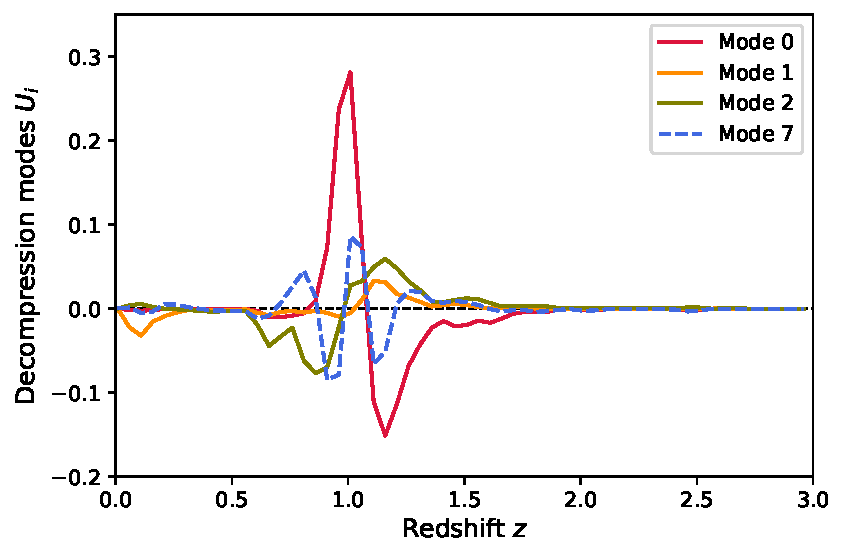
\includegraphics[width=0.6\textwidth]{modes.pdf}
  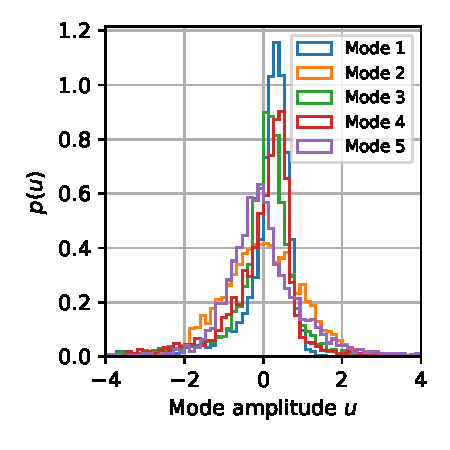
\includegraphics[width=0.38\textwidth]{uhist.pdf}
\caption{At left are plotted the modes, or rows of the decompression
  matrix $\matD$ in \eqq{UU}, that are derived by our method for $\vecn.$
 At right are shown the distributions of the coefficients
  $\vecu$ of the 5 modes that are found by compressing the input
  samples.  Some of the five are substantially non-Gaussian.}
\label{fig:modes}
\end{figure}

The left-hand panel of Figure~\ref{fig:modes} plots the 5 retained
modes of variation of $n(z),$ \ie\ the rows of the decompression
matrix $\matD$ in \eqq{UU}.   Recall that each mode will be multiplied by
a random deviate $u$ with unit variance and added to the mean $\vecn$
to yield a sample from the prior.
 Note that although the successively higher-order modes 
are less detectable by the data, they are not necessarily becoming
numerically smaller perturbations to $n(z)$.

The right-hand panel of Figure~\ref{fig:modes} plots the distributions
of the $M=5$ components of the compressed $\vecu$ representations of the
3000 input samples.  Several of them are substantially non-Gaussian,
so a unit-normal prior on $\vecu$ will not faithfully represent the
input samples---a better density estimator is required.  We find in
this case (and in all other DES cases) that it is sufficient to
normalize the marginal distributions of the individual $u_i$
components.  This is done by tabulating a normalizing function $f_i$
for each mode defined by
\begin{equation}
  {\rm CDF}_n\left[ f_i(u_i) \right] = {\rm CDF}(u_i),
\end{equation}
where the left side is the cumulative distribution function of the
unit normal, and the right-hand side is the CDF of the $u_i$ values
obtained from the input samples.  The functions $f_i$ are bijective
and can be stored as a splined lookup table.
Now, the cosmological Markov Chain
is told that there are five parameters $\widetilde{\vecu}$ that have a
unit-normal prior $p(\widetilde{\vecu}).$  This vector defines the
redshift distribution via a 2-step process:
\begin{align}
  u_i & =f_i^{-1}(\widetilde{u}_i); \\
  \vecn & = \matD \vecu.
\end{align}

\textit{Corner plot of $\widetilde{\vecu})$? ?}


The orange violins in Figure~\ref{fig:violins} show the distributions
of the $n(z)$ values that are generated by drawing $\widetilde{\vecu}$
values from a unit Gaussian.  It is clear now that projecting away the
unobservable fluctuations in $n(z)$ has substantially reduced the
variance of the function.  To check whether we have achieved our goal
of leaving the \emph{observable} consequences of the $n(z)$ variation
unchanged, we calculate the distribution of
\begin{equation}
  \chi^2 =  \left[\hatc(\vecq,\vecn) - \hatc(\vecq,\vecn_0) \right]^T
                                            \left[\covm_c^{-1} \hatc(\vecq,\vecn) - \hatc(\vecq,\vecn_0)\right]
\label{eq:chihist}
\end{equation}
for the cases (1) the $\vecn$ are drawn from the input samples, and
(2) are generated using the procedure defined above.  This $\chi^2$
measures the deviation of the model from that implied by the mean
vector $\vecn_0$ at some chosen nominal value of cosmological
parameters $\vecq$ (we also fix the other nuisance parameters of the
DES model for this test).

Figure~\ref{fig:chihist} shows the results: the $\chi^2$ distribution
for the input samples is indistinguishable from that of the samples
generated by our compressed, normalized representation.
The Figure also shows the $\chi^2$ distribution resulting from samples
generated by the method used in the DES Y3 analysis \citep{y3pz}.  In
that case, the $n(z)$ for each galaxy sample was given an \textit{ad
  hoc} variation of the form
\begin{equation}
  n(z) = n_0\left(\frac{z-\Delta\,z}{s}\right),
\end{equation}
with $\Delta z$ and $s$ being ``shift'' and ``stretch'' parameters.
Separable Gaussian priors were assigned to $\Delta z$ and $s$ with
means of 0 and 1, respectively, and standard deviations that equaled
the RMS variation in the mean and width of the input $n(z)$ samples.
In the Figure we can see that the shift-stretch model does not in fact
reproduce the size of the deviations in the $\vecc$ observables that
is implied by the original samples.

\begin{figure}
  \center
  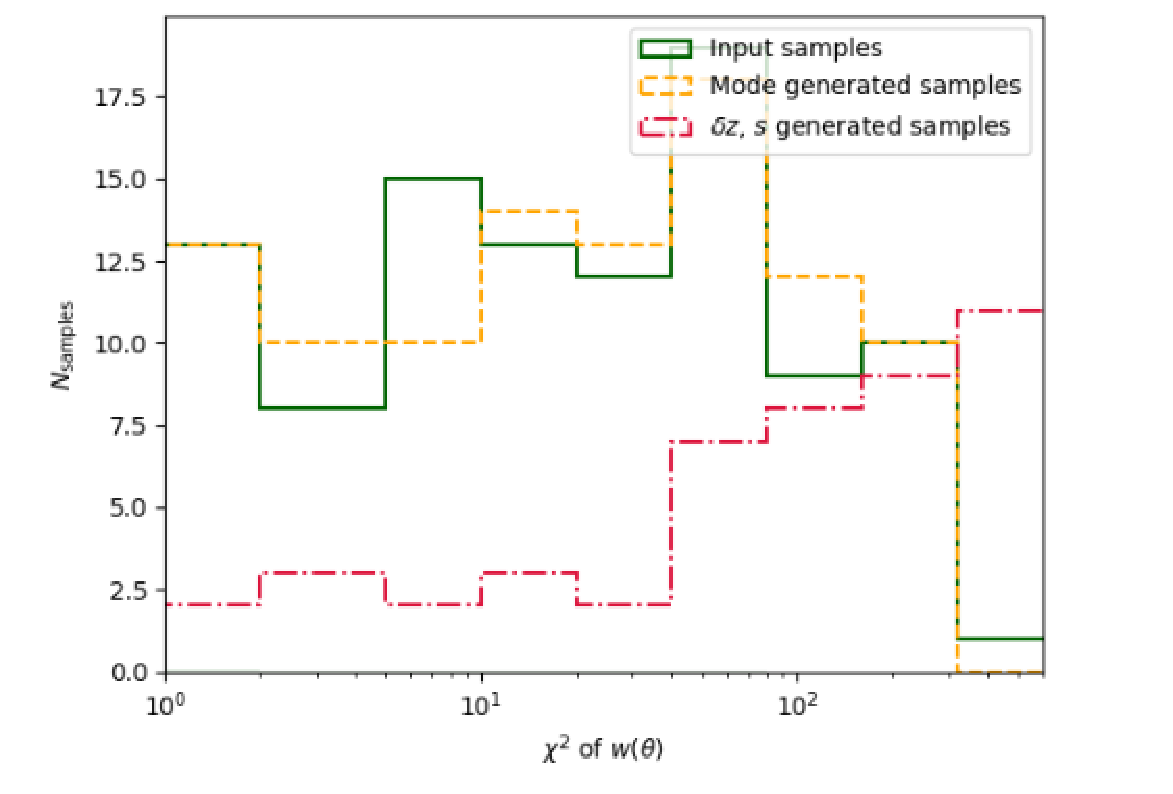
\includegraphics[width=0.6\textwidth]{chihist.pdf}
\caption{The histograms show the deviations of the predicted observable $w(\theta)$ quantities in
  DES Y6 cosmological analysis, as measured by the $\chi^2$ in
  \eqq{eq:chihist}, as we allow the $n(z)$ parameters to vary.  The
  ??? histogram shows the variation using the original 3000 samples of
  $n(z)$ produced by the photometric and clustering redshift studies.
  The ??? histogram results from
  drawing 5-dimensional $\widetilde{\vecu}$ values from a unit
  Gaussian and decompressing them into $n(z)$ realizations using our
  method.  This lower-dimensional model for the prior on $n(z)$
  reproduces the original samples' result very well.  By comparison,
  a \textit{ad hoc} prior for $n(z)$ which reproduces the variations in only the mean
  and width of the input $n(z)$ samples is less accurate in preserving
  the fluctuations in the observable quantity under the
  prior. \textbf{Prelim version of figure.} }
\label{fig:chihist}
\end{figure}


  \begin{acknowledgments}


G.M.B. acknowledges support from NSF grant AST-2205808 and \ldots.

\end{acknowledgments}
\begin{thebibliography}{dummy}
%\bibliography
%\bibliographystyle{aasjournal}
\bibitem[Cordero et al.(2022)]{hyperrank} Cordero, J.~P., Harrison, I., Rollins, R.~P., et al.\ 2022, \mnras, 511, 2170. doi:10.1093/mnras/stac147

\bibitem[Hadzhiyska et al.(2020)]{hans} Hadzhiyska, B., Alonso, D., Nicola, A., et al.\ 2020, \jcap, 2020, 056. doi:10.1088/1475-7516/2020/10/056

\bibitem[Yin et al.(2025)]{y6pz} Yin, B. et al.\ 2025 (PZ paper)
\bibitem[d'Assignies et al.(2025)]{y6wz} d'Assignies, W. et al.\ 2025 (WZ paper)
\bibitem[Giannini et al.(2025)]{y6gg} Giannini, G. et al.\ 2025 (lenses paper)
  
\end{thebibliography}

\end{document}
